%% -*- coding:utf-8 -*-
\chapter{\LaTeX}


\section{Installation of the \texttt{langsci} class}

The \latex class for typesetting Language Science Press books was developed by Timm
Lichte\aimention{Timm Lichte} with
help be Berthold Crysmann\aimention{Berthold Crysmann} and me\aimention{Stefan M{\"u}ller}. It can be downloded from the GitHUB\is{GitHUB} repository at: \url{https://github.com/langsci/latex}
You can download the classes directly from the given web page or use the following git commands to
create a local copy of the repository:
\begin{verbatim}
git init
git clone https://github.com/langsci/latex.git 
\end{verbatim}
If you are using \texttt{git}, you can update your installation by executing the following command:
\begin{verbatim}
git pull origin
\end{verbatim}

Place all files and subdirectories from this repository into your local working directory.

\section{Using the \texttt{langsci} class}

Once you installed the classes in your system, you may look at the file \texttt{test.tex} to see how
a book can be typeset. The code of this book is available in the directory \texttt{Guidelines}. Once
you set up your \latex files you can compile them by calling 
\begin{verbatim}
xelatex yourfilename.tex
\end{verbatim}

%\DescribeMacro{\BackTitle}


\subsection{Class options}

A \latex document starts with a specification of a document class. Usually this is a class for
books, articles, or technical reports. \lsp has a special class that is called \texttt{langsci} and is
based on the book class from the KomaScript package. Several options can be passed to the class. The
following code shows how the class is loaded and how options are set. 


\begin{verbatim}
\documentclass[series=labphon,
               number=1,
               isbn=978-3-944675-01-5,
               url=http://langsci-press.org/catalog/book/16,
               output=long]{langsci}            
\end{verbatim}

The options are explained in the following paragraphs.


\subsubsection{\texttt{series}}

The\isoption{series} name of the series in which a book is published has to be passed to the langsci package. This will ensure that the name of
the series is put on the cover and the right color for your series will be
selected. Table~\vref{table-series} provides an overview of the series that are established as of
\today.
\begin{table}[htbp]
\caption{\label{table-series}Series of \lsp as of \today}
\centerline{%
\begin{tabular}{ll}\hline\hline
Option  & Full Name\\\hline
eotms   & Empirically Oriented Theoretical Morphology and Syntax\\
eotmsig & Implemented Grammars\\
sidl    & Studies in Diversity Linguistics\\
algad   & African Language Grammars and Dictionaries\\
tmnlp   & Translation and Multilingual Natural Language Processing\\
lnls    & Lecture Notes in Language Sciences\\
nc      & Monographs on Comparative Niger-Congo\\
labphon & Studies in Laboratory Phonology\\
\hline\hline
\end{tabular}
}
\end{table}



\subsubsection{\texttt{number}}

Authors\isoption{number} will be informed by their editor about the number that their book has in the series. This
number is passed with the \texttt{number} option to the langsci class.

\subsubsection{\texttt{isbn}}

Once\isoption{isbn} a manuscript is accepted, authors have to sign a publication agreement with the FU Library (see
Chapter~\ref{chap-publication}). Then they will get an ISBN, which has to be passed to the langsci class.

\subsubsection{\texttt{url}}

When\isoption{url} a manuscript is submitted to \lsp the submission gets a number and there will be a
corresponding URL. This URL has to be passed to the langsci class, since it will be part of the
copyright information of the book.

\subsubsection{\texttt{output}}

There\isoption{output} are three options for output: \texttt{long}, \texttt{short}, and \texttt{inprep}. If you pass
\texttt{long} to the langsci class, all pages are printed. This includes front and backpane of the
cover and also its spine. If the option \texttt{short} is used, the cover pages are omitted. This
document version is much more printer friendly since the colored pages are not included.

The option \texttt{inprep} suppresses everything that refers to \lsp. This gives authors the
possibility to write their book using the \lsp classes and styles prior to submission. They may then
distribute the manuscript without revealing their intention to submit to \lsp.

\subsubsection{\texttt{smallfont}}

\lsp\isoption{smallfont} books are typeset with an 11pt font. Those books that would be longer than 500 pages should be
typeset with the \texttt{smallfont} option, which selects a 10pt font.

\subsubsection{\texttt{draftmode}}

Since\isoption{draftmode} \lsp does not have any commercial interest you can put your book on webpages and distribute it
freely. We encourage authors to do this in order to discuss the work and improve it before final
publication. If authors want to circulate prefinal versions, they can use the option
\texttt{draftmode}. This prints a large watermark onto the first page and adds a footer to ever page
that informs the reader about the fact that he is reading a draft and the date and time of the
creation of the draft.


\subsubsection{\texttt{copyright}}

Usually \lsp books are published under the Creative Commons license CC-BY. However, there are rare
cases where other licenses are required (for instance for translations of books that were published
with another publisher who has the rights for the original version). For such cases, there is the
\isoption{copyright} the \texttt{copyright} option. One can pass any other CC license string to the
\latex class in the following way:
\begin{verbatim}
copyright=CC-BY-ND
\end{verbatim}


\subsection{Commands}

You can specify a title with the \verb+\title+\iscommand{title} command (\latex standard). In addition the langsci
class provides a command for specifying a subtitle (\verb+\subtitle+\iscommand{subtitle}). The author of a book is
specified by \verb+\author+\iscommand{author}. A separate page with a dedication can be inserted by \verb+\dedication+\isoption{dedication}.

The title of the book that goes to the back of the book is specified by \iscommand{BackTitle}\verb+\BackTitle+ and the
cover text on the back is provided by \verb+\BackBody+\iscommand{BackBody}.


\section{Workflow}

\subsection{Compiling the document}
\label{sec-latex-compilation}

There are various tools for all existing platforms that help authors/typesetters compiling the
documents and creating indices and references. The following commands can be called explicitly from
the commandline in Unix-based systems:
\begin{fitverb}
xelatex -no-pdf yourfilename
bibtex -min-crossrefs=200 yourfilename
xelatex -no-pdf yourfilename
bibtex -min-crossrefs=200 yourfilename
xelatex yourfilename -no-pdf
correct-toappear
correct-index
makeindex -o yourfilename.ind yourfilename.idx
makeindex -o yourfilename.lnd yourfilename.ldx
makeindex -o yourfilename.wnd yourfilename.wdx
LSP/bin/reverse-index <yourfilename.wdx >yourfilename.rdx
makeindex -o yourfilename.rnd yourfilename.rdx
\rm yourfilename.adx
authorindex -i -p yourfilename.aux > yourfilename.adx
sed -e 's/}{/|hyperpage}{/g' yourfilename.adx > yourfilename.adx.hyp
makeindex -o yourfilename.and yourfilename.adx.hyp
xelatex yourfilename
\end{fitverb}

\noindent
These commands do the following: they run the documents through \xelatex, call \bibtex, create the
indices using \texttt{makeindex}, and create a reverse index of expressions and an author index.

Everytime \xelatex is run it writes information about the sections and figures and son on auxiliary
files. These auxiliary files are read in when \xelatex runs again. They are used by \xelatex to create a
table of contents and by \bibtex to create the list of references. Due to the insertion of a table of
contents the page numbering may change. Therefore it is necessary to run \xelatex several times to
get a stable document.

We decided not to use the crossreferencing\is{crossreferencing} facility that \bibtex provides. Crossreferencing saves
space if several papers in the same edited volume are cited, but is opaque for indexing tools like
google scholar. Crossreferencing is disabled by the command option \verb+-min-crossrefs=200+ that is
passed to the \texttt{bibtex} command.

\subsection{Makefiles}

Of course nobody wants to type in the commands mentioned in Section~\ref{sec-latex-compilation} by
hand. Instead a Makefile\is{Makefile}\is{make} can be used. You will find an example Makefile in the
github repository in the directory that also contains the code for this book.\footnote{
  \url{https://github.com/langsci/latex/tree/master/Guidelines}, 16.02.2014.
}


\subsection{Using includes}

\subsection{Version control}


\section{Document structure}




\subsection{References}

\lsp uses the \texttt{natbib}\ispackage{natbib} package together with \bibtex\is{bibtex@\bibtex} and the \bibtex style \texttt{unified.bst}.


\subsection{Citation}

As was explained in Section~\ref{sec-references-authors} citations that provide a page number are
given required to be in the format Author (1975: 312) rather than Author (1975: p.\,312). If authors
want their text to be copy\&paste-proof, they can define the command \verb+\page+ and cite as
follows:
\begin{verbatim}
\citet[\page 312]{Author1975a}
\end{verbatim}
For \lsp \verb+\page+ would be:
\begin{verbatim}
\newcommand{\page}{}
\end{verbatim}
For other publications authors can use the following
\begin{verbatim}
\newcommand{\page}{p.\,}
\end{verbatim}
In case several pages are cited, the page numbers should be passed to cite as follows:
\begin{verbatim}
\citet[\page 312, 740, 756--758]{Author1975a}
\end{verbatim}


\subsection{Crossreferencing}

You may use \verb+(\mex{1})+\iscommand{mex} to refer to the following example and \verb+(\mex{0})+ to the preceeding
example. You can also pass smaller numbers or larger numbers to \verb+\mex+ but I would suggest not
to do this since often text blocks are inserted between the example and its description and then
references are broken. Furthermore the standard referencing mechanism creates hyperlinks to the
example sentences and depending on your viewer this gives you a nice preview of the referenced
material, which you do not get with \verb+\mex+. See Figure~\vref{fig-preview-of-hyperlink-with-skim} for an example for such a preview.
\begin{figure}[htbp]
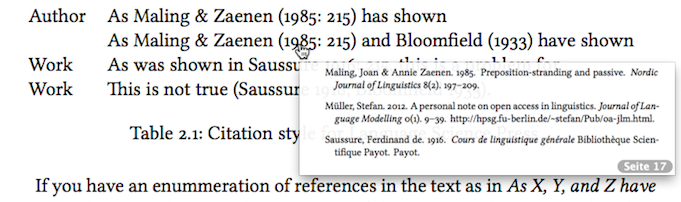
\includegraphics[width=\linewidth]{crossref.png}
\caption{\label{fig-preview-of-hyperlink-with-skim}Hyperlinked reference allow a preview in some viewers}
\end{figure}


There should not be a linebreak in something like \emph{Section~4}. This is achieved by using an explicit
whitespace: \verb+Section~\ref{sec-examples}+ This also makes sure that \latex is not inserting too
much space when material is distributed in a line.

\subsection{Indexes}

The\is{index|(} \lsp class is set up in a way that an author index is created automatically. If you want to add
an author that is not cited (for instance in the acknowledgements), you can do this by calling
\verb+\aimention{Zappa, Frank}+.\aimention{Zappa, Frank}\iscommand{aimention}

You may enter items into the subejct index by calling \verb+\is+, for example 
\begin{verbatim}
\is{word}
\end{verbatim}

Regions can be specified by appending \verb+|(+ to the keyword at the beginning of a region and
\verb+|)+ at the end of the region. For instance this section has the index entry
\verb+\is{index|(}+ after the first word of this section and \verb+\is{index|)}+ at the very end of
this section. If this rather brief section happens to be set on one page, \latex enters one page
number into the index. If there is a pagebreak in the middle of this section, a region is entered
into the index.

If you mention a language, you may add it to the language index: 
\begin{verbatim}
\il{Mandarin Chinese}
\end{verbatim}
If you are working in a theory that uses features (like LFG or HPSG), you may use \verb+\isfeat+ to enter
features into the subject index. \verb+\isfeat{comps}+\isfeat{comps} would enter the \compsf into the subject
index. The typesetting of the feature name in {\sc small caps} will be done automatically.

Words (or stems) can be entered into a special index by using \verb+\iw+. For instance,
\verb+\iw{Mann}+ enters the word \emph{Mann}\iw{Mann} in to the index of expressions.

Authors working in the area of morphology may find a reverse index of expressions useful. For
instance, if one wants to find all references to words ending on \suffix{ung} (as for instance \emph{Besprechung}\iw{Besprechung}, \emph{Lesung}\iw{Lesung},
\emph{Sitzung}\iw{Sitzung}, or \emph{Vorlesung}\iw{Vorlesung}), one can look them up
in the reverse index of expressions easily.

All these index commands can also be used in footnotes.\footnote{
  The commands are set up in a way that automatically distinguishes between index entries in
  footnotes and outside of footnotes. For instance the call of \texttt{$\backslash$iw\{Mann\}} for the word
  \emph{Mann}\iw{Mann} causes a special marking in the expression index.
}

All index entries are hyper-linked to the respective pages.

Indexes are inserted at the end of the document by specifying a subset of the following calls:
\begin{verbatim}
\clearpage
\pdfbookmark[0]{Index}{Index}
\pdfbookmark[1]{Expression index}{Expression index}
\printindex[wrd]
\pdfbookmark[1]{Reverse expression index}{Reverse expression index}
\printindex[rwrd]
\pdfbookmark[1]{Name index}{Name index}
\printindex[aut]
\pdfbookmark[1]{Language index}{Language index}
\printindex[lan]
\pdfbookmark[1]{Subject index}{Subject index}
\printindex
\end{verbatim}

While working at a manuscript it can be practical to see index entries in the margins. Index entries may be
switched on by specifying \verb+\proofmodetrue+ in the preamble of the
document.\iscommand{proofmodetrue} The following specification checks whether the option
\texttt{draftmode}\isoption{draftmode} of the \texttt{langsci} is used and displays the index entries in the margin if
this is the case:
\begin{verbatim}
\iflsDraft
\proofmodetrue
\fi
\end{verbatim}


\is{index|)}

\subsection{Hyphenation}

There is a special draft mode that can be used for the preparation of manuscripts. It can be enabled
by passing the option \texttt{draftmode} to the langsci class. In draftmode words that could not be
hyphenated automatically stick out in the right margin. Such problematic words are marked with a
black box so that they can be detected easily. You can fix such problems by inserting explicit
hyphenation rules in a word. This is done by \verb+\-+, for example \verb+weath\-er+. However, this
method is dispreferred since it only affects one occurrence of the word rather than all occurrences in
the current and further documents. The right way to deal with hyphenation issues is to put your
hyphenation preferences into a file and include this file in all your publications. 

\begin{verbatim}
\hyphenation{
Ajd-ukie-wicz
Prze-piór-kow-ski
To-ma-sel-lo
To-ron-to
trans-for-ma-tions-gram-ma-ti-sches
Tü-bing-en
Um-welt-ver-gif-tung
Ver-lags-buch-hand-lung
West-deut-scher
Wis-sen-schaft-liche
weath-er
}
\end{verbatim}

%xxx xxxxxxxxxxxxxxxxx xxxxxxxxxxxx xxx xxxxxxxxxx xxxxxxxxxxx Wirtschaftswunder.
%
%xxx xxxxxxxxxxxxxxxxx xxxxxxxxxxxx xxx xxxxxxxxxx xxxxxxxxxxx Wissenschaftliche.



\section{Packages specific for linguistics}

There is a huge amount of packages that can be used for various purposes. \citew{MG2013a} is a good
reference book. This section discusses some aspects of some packages that are relevant for
linguistics. Every \latex package comes with a documentation and users should consult these
documentations too. The purpose of this section is to point users to the packages that we think
serve their purpose best and that are compatible with other packages and the \lsp classes, as this
book proves.

\subsection{Glossed examples}

Glossed\is{glossing|(}\ispackageb{lsp-gb4e} examples are typeset with a modified version of the \texttt{gb4e}\ispackage{gb4e} package by Craig
Thiersch\aimention{Craig Thiersch}. The modified package is called \texttt{lsp-gb4e}. It is contained in the styles directory
that is delivered with the \lsp \latex calsses. It differs from the original package in loading a
version of \texttt{gloss} that was modified by Alexis Dimitriadis\aimention{Alexis Dimitriadis} in order to be compatible with
\texttt{jambox} (see Section~\ref{sec-jambox}).

Simple examples like (\mex{1}) can be typeset as shown below.
\ea
\iw{Mann}\iw{schlafen}
\gll Der Mann schläft.\\
     the man  sleeps\\
\glt `The man sleeps.'
\z
\begin{verbatim}
\ea
\gll Der Mann schläft.\\
     the man  sleeps\\
\glt `The man sleeps.'
\z
\end{verbatim}
Lists of examples can be typeset with \verb+\eal+ and \verb+\zl+ respectively. The example in
(\mex{1}) shows how the sentences can be aligned properly:
\eal
\ex[]{
\iw{Linguist}\iw{Nobelpreis}\iw{glauben}
\gll Ich glaube dem Linguisten nicht, einen Nobelpreis gewonnen zu haben.\\
     I believe the linguist not a Nobel.prize won to have\\
\glt  `I don't believe linguist's claim that he won a Nobel prize.'
}
\ex[*]{
\gll Dem Linguisten einen Nobelpreis  glaube  ich nicht gewonnen zu haben.\\
     the linguist   a     Nobel.price believe I   not   won      to have\\
}
\zl
\begin{fitverb}
\eal
\ex[]{
\gll Ich glaube  dem Linguisten nicht, einen Nobelpreis  gewonnen zu haben.\\
     I   believe the linguist   not    a     Nobel.prize won      to have\\
\glt  `I don't believe linguist's claim that he won a Nobel prize.'
}
\ex[*]{
\gll Dem Linguisten einen Nobelpreis  glaube  ich nicht gewonnen zu haben.\\
     the linguist   a     Nobel.price believe I   not   won      to have\\
}
\zl
\end{fitverb}

If you want to add a footnote\is{footnote|(} that provides the source of an example as in (\mex{1}), you can do
this as follows:
\ea
\gll Piloten         fik frataget    sit certifikat\footnotemark\\
     pilot.{\sc def} got deprived.of his license\\
\footnotetext{KorpusDK.}
\glt `The pilot was deprived of his license to fly.'
\z 
\begin{verbatim}
\ea
\gll Piloten         fik frataget    sit certifikat\footnotemark\\
     pilot.{\sc def} got deprived.of his license\\
\footnotetext{KorpusDK.}
\glt `The pilot was deprived of his license to fly.'
\z 
\end{verbatim}
Please call the \verb+\footnotetext+ command before the translation, since otherwise the
footnotetext may be typeset on a page that is different from the one where the footnotemark is set.\is{footnote|)}

For the typesetting of an additional line with the original script, one may use \verb+\glll+ rather
than \verb+\gll+. (\mex{1}) shows a Chinese example:
\ea
\label{ex-chinese}
\glll 狗       叫     了。\\
      gou3     jiao4   le\\
      dog      bark    ASP/CRS\\
\glt `The dog is barking.'/`The dogs are barking.'
\z

\begin{verbatim}
\ea
\glll 狗       叫     了。\\
      gou3     jiao4   le\\
      dog      bark    ASP/CRS\\
\glt `The dog is barking.'/`The dogs are barking.'
\z
\end{verbatim}


In some subdisciplines of linguistics (e.\,g.\ typology) the examples are written in italics as in the
following example:
\ea
\def\exfont{\normalsize\it}
\gll Piloten         fik frataget    sit certifikat\footnotemark\\
     pilot.{\sc def} got deprived.of his license\\
\footnotetext{KorpusDK.}
\glt `The pilot was deprived of his license to fly.'
\z 
Authors do not have to care for this. The code for typesetting this is exactly the same as for the
variant without italics.
% of course this is not true for the code above ...
The series editor decided whether italics is used or not.

If the series decides to use italics, it has to be ensured that structural markup like brackets are
not typeset in italics:
\ea
\def\exfont{\normalsize\it}
\gll ein {\rm[}interessantes       Beispiel{\rm]}\\
     an  \hspaceThis{[}interesting example\\
\glt `an interesting example'
\z 
\begin{verbatim}
\ea
\gll ein {\rm[}interessantes       Beispiel{\rm]}\\
     an  \hspaceThis{[}interesting example\\
\glt `an interesting example'
\z 
\end{verbatim}
\is{glossing|)}\ispackagee{lsp-gb4e}
%% \inlinetodostefan{
%% The translation should not be separated from the glossed example by a page break.
%% }

In typological series examples often come with the language name and references. The examples on
page~\pageref{ex-typology} are typeset as follows:
\begin{verbatim}
\ea
{\rm Mising\il{Mising} \citep[69]{Prasad91a}}\\
\gll azɔ́në dɔ́luŋ\\
     small village\\ 
\glt `a small village' 
\z

\eal
\ex {\rm Apatani\il{Apanti} \citep[23]{Abraham85a}}\\
\gll aki atu\\ 
     dog small\\ 
\glt ‘the small dog’ 
\ex {\rm Temiar\il{Temiar} \citep[155]{Benjamin76a}}\\ 
\gll dēk mənūʔ\\
     house big\\
\glt ‘big house’ 
\zl
\end{verbatim}


\subsection{\texttt{jam\-box}}
\label{sec-jambox}


The\ispackageb{jam\-box} package \texttt{jambox} by Alexis Dimitriadis\aimention{Alexis Dimitriadis} can be used to provide information about the language of an example or
about a certain other aspect to be highlighted.\il{Maltese}
\settowidth\jamwidth{VSO}
\eal
\ex[]{
\label{ex-ingrid-kielet-ilmazzita}
\gll Ingrid kiel-et il-mazzit-a.\\
     Ingrid eat-{\sc 3sg.f} {\sc def}-black.pudding-{\sc sg.f}\\ \jambox{(SVO)}
\glt `Ingrid ate black pudding.'
}
\ex[]{
Kielet ilmazzita Ingrid. \jambox{(VOS)}
}
\ex[*]{
Kielet Ingrid ilmazzita. \jambox{(VSO)}
}
\ex[]{\label{ex-sov}
Ingrid ilmazzita kielet. \jambox{(SOV)}
}
\ex[]{\label{ex-osv}
Ilmazzita Ingrid kielet. \jambox{(OSV)}
}
\ex[]{
Ilmazzita kielet Ingrid. \jambox{(OVS)}
}
\zl

The call of \verb+\jambox+ has to follow the linebreak after the gloss:
\begin{verbatim}
\ex[]{
\label{ex-ingrid-kielet-ilmazzita}
\gll Ingrid kiel-et il-mazzit-a.\\
     Ingrid eat-3fsg def-black.pudding-fsg\\ \jambox{(SVO)}
\glt `Ingread ate black pudding.'
}
\end{verbatim}
The distance from the right margin can be specified by passing the largest object to be placed in a
jambox to \verb+\settowidth+:

\eal
\settowidth\jamwidth{(German)}
\ex The man reads the book.    \jambox{(English)}
\ex Manden læser bogen.        \jambox{(Danish)}
\ex Der Mann liest das Buch.   \jambox{(German)}
\zl

\begin{verbatim}
\eal
\settowidth\jamwidth{(German)}
\ex The man reads the book.    \jambox{(English)}
\ex Manden læser bogen.        \jambox{(Danish)}
\ex Der Mann liest das Buch.   \jambox{(German)}
\zl
\end{verbatim}
\ispackagee{jam\-box}



\subsection{Trees: \texttt{tikz-qtree}}

Several\ispackageb{tikz-qtree} tree-drawing packages are around and all have their advantages and disadvantages. I
used \texttt{tree-dvips} for decades, but it is incompatible with \xelatex, since it creates
PostScript rather than PDF. Exploring the options I discovered \texttt{tikz-qtree}, which is a
tikz-based\ispackage{tikz} reimplementation of Alexis Dimitriadis'\aimention{Alexis Dimitriadis} \texttt{q-tree}
package. The syntax for drawing trees is rather simple and in comparison to \texttt{tree-dvips} drawing trees
is considerably speeded up. Figure~\vref{fig-the-dog-barks} shows a simple example.
\begin{figure}[htbp]
\centerline{%
\begin{tikzpicture}
\tikzset{level 1+/.style={level distance=2\baselineskip}}
\tikzset{frontier/.style={distance from root=6\baselineskip}}
\Tree[.S
       [.NP 
         [.Det the ]
         [.N   dog ] ]
       [.VP barks ] ]
\end{tikzpicture}
}
\caption{\label{fig-the-dog-barks}Tree for \emph{The dog barks.} drawn with \texttt{tikz-qtree}}
\end{figure}
\begin{fitverb}
\begin{tikzpicture}
\tikzset{level 1+/.style={level distance=2\baselineskip}}
\tikzset{frontier/.style={distance from root=6\baselineskip}}
\Tree[.S
       [.NP 
         [.Det the ]
         [.N   dog ] ]
       [.VP barks ] ]
\end{tikzpicture}
\end{fitverb}

The code below shows how words below a certain node can be put under a triangle as in Figure~\vref{fig-the-dog-barks-abbreviated}.
\begin{figure}[htbp]
\centerline{%
\begin{tikzpicture}
\tikzset{level 1+/.style={level distance=2\baselineskip}}
\tikzset{frontier/.style={distance from root=5\baselineskip}}
\Tree[.S
       [.NP  \edge[roof]; {the dog} ]
       [.VP barks ] ]
\end{tikzpicture}
}
\caption{\label{fig-the-dog-barks-abbreviated}Tree for \emph{The dog barks.} with abbreviated NP}
\end{figure}

\begin{samepage}
\begin{fitverb}
\begin{tikzpicture}
\tikzset{level 1+/.style={level distance=2\baselineskip}}
\tikzset{frontier/.style={distance from root=5\baselineskip}}
\Tree[.S
       [.NP  \edge[roof]; {the dog} ]
       [.VP barks ] ]
\end{tikzpicture}
\end{fitverb}
\end{samepage}
\ispackagee{tikz-qtree} 

\subsection{DRSes: \texttt{drs}}

DRSes\ispackageb{drs} can be typeset using the \texttt{drs} package by Alexis Dimitriadis\aimention{Alexis
  Dimitriadis}. There are various commands that let you typeset simple DRSes, ones with implications
and DRSes with quantifiers. Some examples from the manual are given below:

\bigskip

\drs{x y}{Jones(x) \\ Ulysses(y) \\ x owns y}

\begin{verbatim}
\drs{x y}{Jones(x) \\ Ulysses(y) \\ x owns y}
\end{verbatim}


\drs{x}{Jones(x) \\
      \ifdrs{y}{donkey(y)\\x owns y}
            {z w}{z = x\\ w = y\\ z feeds w}}

\begin{verbatim}
\drs{x}{Jones(x) \\
      \ifdrs{y}{donkey(y)\\x owns y}
            {z w}{z = x\\ w = y\\ z feeds w}}
\end{verbatim}

\drs{X}{ the lawyers(X) \\
        \qdrs{x}{x $\in$ X}
             {every}{x}
             {y}{secretary(y) \\ x hired y}}

\begin{verbatim}
\drs{X}{ the lawyers(X) \\
        \qdrs{x}{x $\in$ X}
             {every}{x}
             {y}{secretary(y) \\ x hired y}}
\end{verbatim}
\ispackagee{drs}

%%%%%%%%%%%%%%%%%%%%%%%%%%%%%%%%%%%%%%%%%%%%%%%%%%%%%%%%%%%%%%%%%%%%%%%%%%%%%%%%%%%%%%%%%%%%%%%%%%%

\subsection{AVMs}

The package for typesetting AVMs that is most widely used is the package \texttt{avm}\ispackage{avm}
by Chris Manning\aimention{Chris Manning}. 

%% This package is described in the following
%% subsection. Section~\ref{sec-lsp-avm} describes AVM macros that were put together by Markus Duda\aimention{Markus Duda}.

%% \subsubsection{\texttt{avm}}

(\mex{1})\ispackageb{avm} shows an example of an AVM typeset with the \texttt{avm} package:
\ea
\label{ex-avm-avm}
\begin{avm}
\[phon   & \< {\it porcupine\/} \>\\
  feat-a & \@{10} \[feat-aa & type-aa\\
                    feat-ab & \< \[ synsem|loc|cat|head & type-aba\\
                                    feat-abc \tpv{type-abc} 
                                  \],
                                  \textup{NP} \>\\
                    \tp{type-a}
                  \]\\
 feat-b & \@{10} type-b\\ 
 \tp{some-type}
\]
\end{avm}
\z



\begin{verbatim}
\begin{avm}
\[phon   & \< {\it porcupine\/} \>\\
  feat-a & \@{10} \[feat-aa & type-aa\\
                    feat-ab & \< \[ synsem|loc|cat|head & type-aba\\
                                    feat-abc \tpv{type-abc} 
                                  \],
                                  \textup{NP} \>\\
                    \tp{type-a}
                  \]\\
 feat-b & \@{10} type-b\\ 
 \tp{some-type}
\]
\end{avm}
\end{verbatim}
%
The command \verb+\tp+ is defined as follows (the code is taken from Detmar
Meurers'\aimention{Detmar Meurers} \texttt{avm+}\ispackage{avm+}):
\begin{verbatim}
% command to fontify the type values of an avm 
\newcommand{\tpv}[1]{{\avmjvalfont #1}}

% command to fontify the type of an avm and avmspan it
\newcommand{\tp}[1]{\avmspan{\tpv{#1}}}
\end{verbatim}

A more complex example is given in (\mex{1}):
\ea
\label{ex-avm-avm}
  \begin{avm}
    {\it word\/} $\rightarrow$
    \[ morphs & $\@{e_1}\bigcirc\cdots\bigcirc\@{e_n}$\\
       morsyn & \@0 $(\@{m_1}\uplus\cdots\uplus\@{m_n})$\\
       rules  & \< \[ morphs & \@{e_1}\\
                      mud & \@{m_1}\\ 
                      morsyn & \@0\], \ldots ,
                    \[morphs & \@{e_n}\\
                      mud    & \@{m_n}\\ 
                      morsyn & \@0\] \>
    \]
  \end{avm}
\z


The code is given below:
\begin{verbatim}
  \begin{avm}
    {\it word\/} $\rightarrow$
    \[ morphs & $\@{e_1}\bigcirc\cdots\bigcirc\@{e_n}$\\
       morsyn & \@0 $(\@{m_1}\uplus\cdots\uplus\@{m_n})$\\
       rules  & \< \[ morphs & \@{e_1}\\
                      mud & \@{m_1}\\ 
                      morsyn & \@0\], \ldots,
                    \[morphs & \@{e_n}\\
                      mud    & \@{m_n}\\ 
                      morsyn & \@0\] \>
    \]
  \end{avm}
\end{verbatim}
With the \texttt{avm} package it is possible to use brackets as they are used in AVMs.

The package has a good documentation and we will not repeat all the details here.
\ispackagee{avm}

%% \subsubsection{\texttt{lsp-avm}}
%% \label{sec-lsp-avm}

%% An alternative way to typeset AVMs is provided in the \lsp style file \texttt{lsp-avm} that contains
%% code by Markus Duda\aimention{Markus Duda} with some adaptions by Stefan Müller\aimention{Stefan
%%   M{\"u}ller}. The AVM in (\ref{ex-avm-avm}) is typeset as follows:

%% \ea
%% \ms[some-type]{
%%   phon   & \phonliste{ porcupine } \\
%%   feat-a & \ibox{10} \ms[type-a]{ feat-aa & type-aa\\
%%                                   feat-ab & \liste{ \onems{ synsem|loc|cat|head \type{type-aba}\\
%%                                                             feat-abc \type{type-abc} },
%%                                   NP }\\ }\\
%%  feat-b & \ibox{10} type-b\\ 
%% }
%% \z

%% %\ea
%% \begin{verbatim}
%% {\it word\/} $\rightarrow$
%%     \ms{ morphs & $\ibox{e_1}\bigcirc\cdots\bigcirc\ibox{e_n}$\\
%%          morsyn & \ibox{0} $(\ibox{m_1}\uplus\cdots\uplus\ibox{m_n})$\\
%%          rules  & \liste{ \ms{ morphs & \ibox{e_1}\\
%%                                mud & \ibox{m_1}\\ 
%%                                morsyn & \ibox{0} }, \ldots ,
%%                           \ms{ morphs & \ibox{e_n}\\
%%                                mud    & \ibox{m_n}\\ 
%%                                morsyn & \ibox{0} } }
%%       }
%% \end{verbatim}


\subsection{OT tableaux}


This\is{Optimality Theory|(}\is{tabular} section just provides some examples of how Optimality Tableaux can be typeset.

\begin{tabular}
       {|lc|c|c|c|}\hline   
      & \textbf{Input}  & Cnstrnt 1  &  Cnstrnt 2& Cnstrnt 3\\ \hline\hline
      & candidate 1     & *!         &           &          \\ \hline
      & candidate 2     &            &  *        &          \\ \hline
\hand & candidate 3     &            &           &  *       \\ \hline
\end{tabular}

\begin{fitverb}
\begin{tabular}
       {|lc|c|c|c|}\hline   
      & \textbf{Input}  & Cnstrnt 1  &  Cnstrnt 2& Cnstrnt 3\\ \hline\hline
      & candidate 1     & *!         &           &          \\ \hline
      & candidate 2     &            &  *        &          \\ \hline
\hand & candidate 3     &            &           &  *       \\ \hline
\end{tabular}
\end{fitverb}

\verb+\hand+ is defined as follows:

\begin{verbatim}
\usepackage{pifont}
\newcommand{\hand}{\ding{43}}
\end{verbatim}
 


\begin{tabular*}{0.95\textwidth}
    {@{\extracolsep{\fill}}|rl||c|c|c|}\hline   
      & \textbf{Input} & Constraint 1 & Constraint 2 & Constraint 3 \\ \hline\hline
      & candidate 1    & *!           &              &              \\ \hline
      & candidate 2    &              &  *           &              \\ \hline
\hand & candidate 3    &              &              &  *           \\ \hline
\end{tabular*}

\begin{fitverb}
\begin{tabular*}{0.95\textwidth}
    {@{\extracolsep{\fill}}|rl||c|c|c|}\hline   
      & \textbf{Input} & Constraint 1 & Constraint 2 & Constraint 3 \\ \hline\hline
      & candidate 1    & *!           &              &              \\ \hline
      & candidate 2    &              &  *           &              \\ \hline
\hand & candidate 3    &              &              &  *           \\ \hline
\end{tabular*}
\end{fitverb}

\begin{tabular}[t]{r|c|c|c|}
\cline{2-4}
      & /qi/  & qi    & qi         \\
\LCC 
      &       &       & \lightgray \\ \cline{2-4}
\hand & [qi]  &       & *          \\ \cline{2-4}
      & [*qi] & *!    &            \\ \cline{2-4}
\ECC
\end{tabular}


\begin{verbatim}
\usepackage{pstricks,colortab}

\begin{tabular}[t]{r|c|c|c|}
\cline{2-4}
      & /qi/  & qi    & qi         \\
\LCC 
      &       &       & \lightgray \\ \cline{2-4}
\hand & [qi]  &       & *          \\ \cline{2-4}
      & [*qi] & *!    &            \\ \cline{2-4}
\ECC
\end{tabular}
\end{verbatim}


\begin{tabular}{|l||c|c|} \hline
          &VO          &OV         \\ \hline\hline
\LCC
          &            &\lightgray \\ \hline
prefixing &Tagalog     &Ma'a       \\ \hline
\ECC
\LCC
           &\lightgray &            \\ \hline
suffixing  &Kwakwala   &Japanese    \\ \hline
\ECC
\end{tabular}

\begin{verbatim}
\begin{tabular}{|l||c|c|} \hline
          &VO          &OV         \\ \hline\hline
\LCC
          &            &\lightgray \\ \hline
prefixing &Tagalog     &Ma'a       \\ \hline
\ECC
\LCC
           &\lightgray &            \\ \hline
suffixing  &Kwakwala   &Japanese    \\ \hline
\ECC
\end{tabular}
\end{verbatim}
\is{Optimality Theory|)}



\subsection{Font issues and right to left scripts}

Since\is{font|(} we are using \xelatex, all fonts that are installed in the cannonical font directories can be
used. We are using the font \texttt{Linux Libertine}, which is unicode-based and contains a lot of
the characters linguists want to use.

\subsubsection{Chinese}
\label{sec-Chinese}

You can enter Chinese\il{Chinese}\is{Chinese Characters} characters directly and mix them with ASCII text without any further markup
provided you load the \texttt{xeCJK}\ispackage{xeCJK} package. We already saw an example in (\ref{ex-chinese}) on
page~\pageref{ex-chinese}. In order to type Chinese text, one has to load the \texttt{xeCJK} package
with the option \verb+indentfirst+ set to \verb+false+ and select an appropriate font:
\begin{verbatim}
\usepackage[indentfirst=false]{xeCJK}
\setCJKmainfont{SimSun}
\end{verbatim}


\subsubsection{Arabic script}

Arabic script\is{Arabic Script}\il{Persian} is the most challenging script for typesetting since it is written from right to left
and contains ligatures. If you load the \texttt{bidi} package, you can mix right to left and left to
right text.\footnote{
  Please have a look at the source code. The verbatim environment has difficulties to display Arabic
  text and hence the call to \texttt{$\backslash$PRL} comes out scrambled.
}

\ea
\PRL{او مرد را دوست نخواهد داشت.}\\
 \gll U      mard rā        dust   naxāhad        dāšt.\\
      He/she man  {\sc dom} friend {\sc neg}.want have\\
\glt `He/she will not love the man.'
\z

%\begin{rtlverbatim}
%\usepackage{fontspec}
\begin{verbatim}
\newfontfamily\Parsifont[Script=Arabic]{XB Niloofar}
\usepackage{bidi}
\newcommand{\PRL}[1]{\RL{\Parsifont #1}}

\ea
\PRL{او مرد را دوست نخواهد داشت.}\\
\gll U      mard rā       dust   naxāhad        dāšt.\\
     He/she man {\sc dom} friend {\sc neg}.want have\\
\glt `He/she will not love the man.'
\z
\end{verbatim}
%\end{rtlverbatim}

\subsubsection{Hebrew}

Hebrew\il{Hebrew|(} is also written from right to left. The characters are part of Linux Libertine, so no extra
font has to be loaded to set examples like (\mex{1}):
\ea
\RL{האישה קוראת ספר.}\\
\gll   ha-'iša          qore't                            sefer.\\
       {\sc def}-woman  read.{\sc pres}.{\sc f}.{\sc sg}  book\\
\glt `The woman is reading a book.'
\z
\begin{fitverb}
\ea
\RL{האישה קוראת ספר.}\\
\gll   ha-'iša          qore't                            sefer.\\
       {\sc def}-woman  read.{\sc pres}.{\sc f}.{\sc sg}  book\\
\glt `The woman is reading a book.'
\z
\end{fitverb}
\il{Hebrew|)}

\subsubsection{IPA symbols}

The\is{IPA symbols|(} IPA symbols are part of the Linux Libertine font and hence can be entered into the document
directly. The IPA unicode symbols can be created online at
\url{http://ipa.typeit.org/full/}. (\mex{1}) shows some examples:
\ea
ɓ ɐ ʁ ɾ ɻ ʃ ʂ θ~  t͡ʃ~  t͡s  ʈ ʊ ʊ̈ ʉ ʌ ʋ ʍ ɯ ɰ χ ʎ ɣ ʏ ɤ ʒ ʐ ʑ ʔ ʕ ʢ ʡ ɑ̃ ɔ ˧ ˨ ˩ ˩˥ ˥˩ ˦˥
\z
% ⱱ does not work  
If you find symbols that are not covered by the font, please use the \texttt{tipa} package.
\is{font|)}\is{IPA symbols|)}

\section{Bells and whistles}

\subsection{\texttt{varioref}}

\texttt{varioref}\ispackageb{varioref} is loaded by the \lsp class file. You can use \verb+\vref+\iscommand{vref} to refer to floating
objects like figures and tables. \latex automatically determines whether the floating object is on
the same page or further away. If the float is on the next page and the next page is to the right of
the current page, \latex will insert an appropriate text like \emph{on the facing page}. If we are
on a right page, \latex will insert something like \emph{on the next page} or \emph{on the facing page}. If the float is further
away, a page number will be provided.
\ispackagee{varioref}

%Please use \verb+\vref+ for the first reference to a float only.


\subsection{\texttt{german} for hyphenation}

If\is{hyphenation|(}\ispackageb{german} you write things like \verb+head-driven+ or very long paths like
{\sc snysem$|$""loc$|$""cat$|$""head$|$""mod$|$""loc}, \LaTeX{} does not do hyphenation
(in the part following the dash).

\verb+german.sty+ provides additional markup that allows for proper hyphenation:
\begin{verbatim}
head"=driven

{\sc snysem$|$""loc$|$""cat$|$""head$|$""mod$|$""loc}
\end{verbatim}
With this markup even long paths like {\sc snysem$|$loc$|$cat$|$""head$|$""mod$|$""loc$|$""cat$|$""head}
are typeset properly. Alternatively you my write
\begin{verbatim}
{\sc snysem$|$\-loc$|$\-cat$|$\-head$|$\-mod}
\end{verbatim}
which introduces a dash at the place of the linebreak:
{\sc snysem$|$\-loc$|$\-cat$|$\-head$|$\-mod$|$\-loc$|$\-cat$|$\-head}.

If you use \verb+german.sty+ for a book whose primary language is not German, do not forget to
specify the language you are using. For example, if your book is in US English you have to specify
the following:
\begin{verbatim}
\selectlanguage{USenglish}
\end{verbatim}
Otherwise the section name for references comes out in German.
\is{hyphenation|)}\ispackagee{german}

\subsection{Resizing large objects}

Trees and AVMs often are too big to fit onto one page. The \texttt{langsci} comes with commands for
shrinking large objects. You may pass your complex object as an argument to \texttt{\oneline} and
this will scale the object to \verb+\linewidth+ (the remaining space on the current line). There is
a more clever version of this command: \verb+\centerfit+. This command checks whether there is
enough space for an object and if this is the case it centers it in the line. If the object is
larger than the \verb+\linewidth+, it is resized to fit the line. This is very handy for typesetting
figures. You may copy and paste figures to other documents with a different text width without any
adaptations.


%% \begin{figure}[htb]
%% \centerfit{%
%% \begin{tikzpicture}
%% \tikzset{level 1+/.style={level distance=3\baselineskip}}
%% \tikzset{level 2+/.style={level distance=5\baselineskip}}
%% \tikzset{level 3+/.style={level distance=6\baselineskip}}
%% \tikzset{level 4/.style={level distance=7\baselineskip}}
%% \tikzset{level 5+/.style={level distance=5\baselineskip}}
%% \tikzset{frontier/.style={distance from root=26\baselineskip}}
%% %% \Tree[.{\ms[np-passive-cx]{ vform & passive \\
%% %%                             subj & \sliste{ NP\ind{1} }\\[2mm]
%% %%                             comps & \sliste{ (PP[\type{by}]\ind{2}) }\\
%% %%                           } }
%% %%         \ms{ vform & psp \\
%% %%              subj & \sliste{ NP\ind{2} }\\[2mm]
%% %%              comps & \sliste{ NP\ind{1} } 
%% %%            } ]
%% \Tree[.S
%%        [.{\ibox{1} NP\ind{2}} \edge[roof]; {the boy} ]
%%        [.VP\feattab{
%%                  \subj  \sliste{ \ibox{1} NP\ind{2} },\\
%%                  \comps  \sliste{  }}
%%          [.V\feattab{
%%                  \subj  \sliste{ \ibox{1} NP\ind{2} },\\
%%                  \comps  \sliste{ \ibox{3} }} was ]
%%          [.{\ibox{3} VP\feattab{
%%                  \vform \type{passive},\\
%%                  \subj  \sliste{ \ibox{1} NP\ind{2} },\\
%%                  \comps  \sliste{ }}} \edge node[auto=left]{Passive Construction};
%%            [.V\feattab{
%%                  \vform \type{psp},\\
%%                  \subj  \sliste{ NP },\\
%%                  \comps  \sliste{ NP\ind{2} }} 
%%              [.V\feattab{
%%                  \vform \type{psp},\\
%%                  \subj  \sliste{ NP },\\
%%                  \comps  \sliste{ NP\ind{2}, \ibox{4} }} given ] \edge node[auto=left]{Schema for Passive Participles};
%%              [.{\ibox{4} NP} \edge[roof]; { the ball } ] ] ] ] ] 
%% \end{tikzpicture}
%% }
%% \caption{\label{fig-the-boy-was-given-the-ball-tseng}Analysis of \emph{The boy was given the ball} according to \citet{Tseng2007a}}
%% \end{figure}


\subsection{Rotating figures and tables}
 

\subsection{\texttt{xspace} and abbreviations}

\ispackage{xspace}

\subsection{\texttt{todonotes}}

\ispackage{todonotes}

%% \section{Software}

%% \begin{itemize}
%% \item BibDesk
%% \item JabRef
%% \end{itemize}


\subsection{Style files and multiple projects}

Paths, shell variables \ldots

\section{Things you should not do}

\begin{itemize}
\item Please do not use explicit line breaks to mark a new paragraph. Paragraphs are marked by an empty
line in the text.
%\item Please do not 
\end{itemize}

\section{Checklist for typesetters/authors using \latex}
\label{sec-check-typesetters}

\begin{itemize}
\item Does your book compile without error messages? (Sounds trivial, but some tools just skip
  \latex errors)
\end{itemize}


%      <!-- Local IspellDict: en_US-w_accents -->
